\section{Neutrino Oscillations}

\subsection{Neutrinos as Fundamental Particles}

\begin{frame}{What are Neutrinos?}
  \begin{minipage}[\textheight]{\textwidth}
  \begin{columns}[T]

  \begin{column}{0.6\textwidth}
  \begin{figure}
  %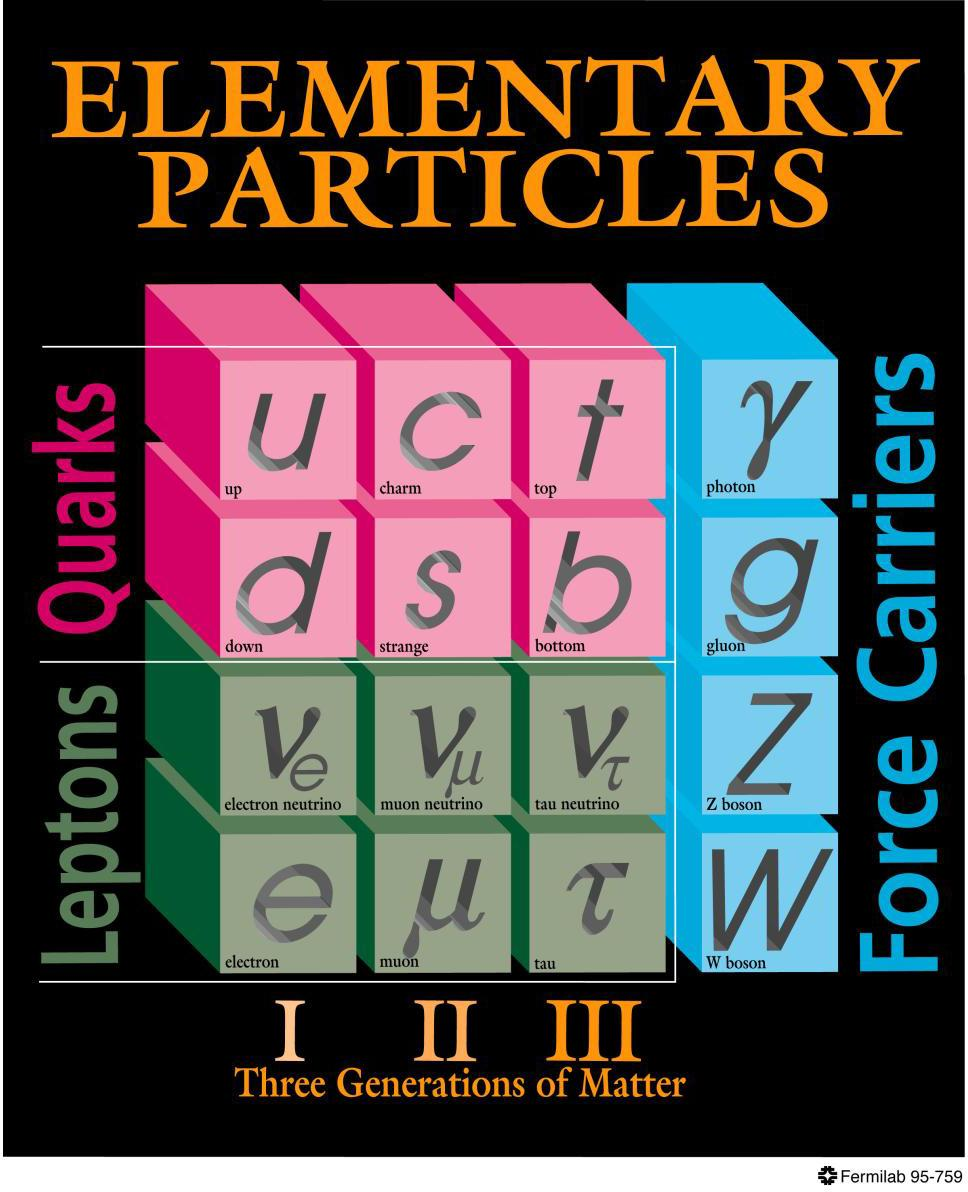
\includegraphics[width=0.9\linewidth,height=0.8\textheight,keepaspectratio]{assets/elementary-particles}
  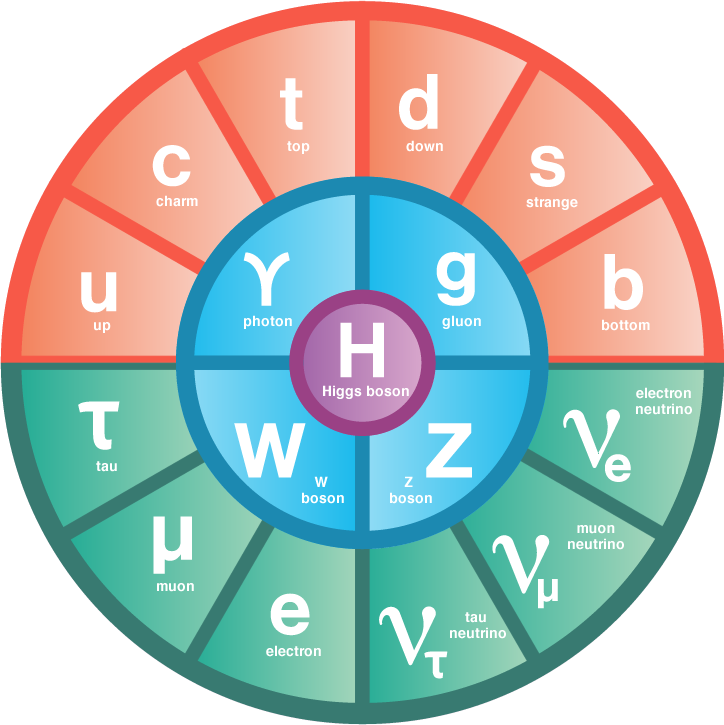
\includegraphics[width=0.9\linewidth,height=0.8\textheight,keepaspectratio]{assets/standard-model}
  \caption*{Elementary particles. \\ Source: symmetrymagazine.org} % http://www-d0.fnal.gov/Run2Physics/WWW/results/final/TOP/T06C/T06C.html
  \end{figure}
  \end{column}

  \begin{column}{0.4\textwidth}


      \begin{itemize}
      \item[] Neutrinos are
      \item fermions,
      \item electrically neutral,
      \item three flavors,
      \item non-vanishing mass.
      \end{itemize}



  \only<1-1>{
  \begin{figure}
  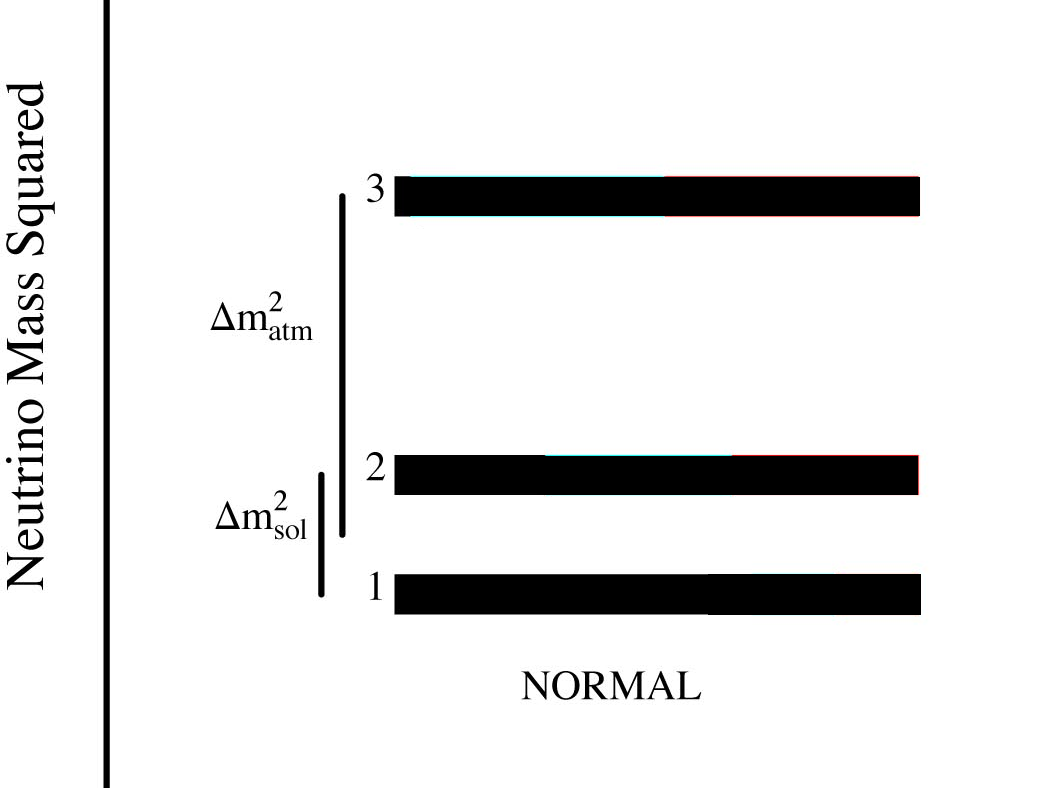
\includegraphics[height=0.4\textheight]{assets/neutrino-mass-normal-hierarchy-simple.png}
  \caption*{Adapted from Olga Mena \& Stephen Parke (2004)}
  \end{figure}
  }

  \only<2-2>{
  \begin{figure}
  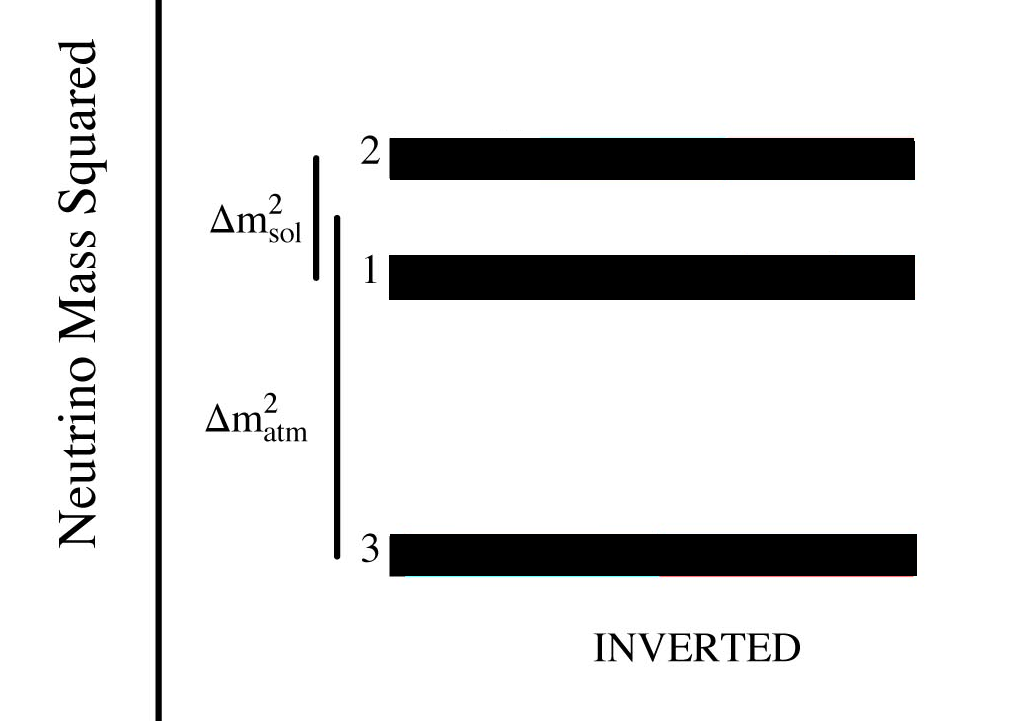
\includegraphics[height=0.4\textheight]{assets/neutrino-mass-inverted-hierarchy-simple.png}
  \caption*{Adapted from Olga Mena \& Stephen Parke (2004)}
  \end{figure}
  }

  \end{column}


  \end{columns}
  \end{minipage}

\end{frame}


%%%%% Neutrino Oscillations %%%%%%%%%

\subsection{Why Do Neutrinos Oscillate}

% For every picture that defines or uses external nodes, you'll have to
% apply the 'remember picture' style. To avoid some typing, we'll apply
% the style to all pictures.
\tikzstyle{every picture}+=[remember picture]

% By default all math in TikZ nodes are set in inline mode. Change this to
% displaystyle so that we don't get small fractions.
\everymath{\displaystyle}


\begin{frame}{Why Do Neutrinos Oscillate?}

\begin{tcolorbox}[box align=center,halign=center,valign=center, standard jigsaw,opacityback=0, coltext=white]
Two flavor senario
\end{tcolorbox}

Flavor states are different from mass states.

\begin{equation*}
\begin{pmatrix}
\psi_e\\
\psi_\mu
\end{pmatrix} = \begin{pmatrix}
\cos \theta_{\mathrm v} & \sin\theta_{\mathrm v} \\
-\sin \theta_{\mathrm v} & \cos \theta_{\mathrm v}
\end{pmatrix}\begin{pmatrix}
\psi_1\\
\psi_2
\end{pmatrix}
\end{equation*}


$\theta_{\mathrm v}$: vacuum mixing angle

\end{frame}



\begin{frame}[fragile]{Why Do Neutrinos Oscillate?}
\setbeamercovered{invisible}





\begin{tcolorbox}[title=Equation of Motion, standard jigsaw, opacityback=0, coltext=white]

\begin{equation*}
i\partial_x \begin{pmatrix}
\psi_e\\
\psi_\mu
\end{pmatrix} = \mathbf{H}\begin{pmatrix}
\psi_e\\
\psi_\mu
\end{pmatrix}
\end{equation*}

\end{tcolorbox}

\pause

\begin{tcolorbox}[standard jigsaw, opacityback=0,coltext=white]
\begin{equation*}
\mathbf{H} = \frac{\omega_{\mathrm v} }{2}\left( - \cos 2\theta_{\mathrm v } \boldsymbol{\sigma}_3  + \sin 2\theta_{\mathrm{v}} \boldsymbol{\sigma}_1\ \right)
\end{equation*}


\begin{itemize}
\item  Mixing angle $\theta_{\mathrm v}$
\item  Oscillation frequency:
\begin{equation*}
\omega_{\mathrm v} = \frac{\delta m^2}{2E}=\frac{m_2^2 - m_1^2}{2E}
\end{equation*}

\end{itemize}


\end{tcolorbox}






\end{frame}



\begin{frame}{Flavor Isospin}
\setbeamercovered{invisible}








\begin{columns}[T]
\begin{column}{0.5\textwidth}


Hamiltonian: $\mathbf H = - \frac{\vec{\boldsymbol{\sigma}} }{2}\cdot \vec H$


Flavor isospin: $\vec s = \Psi^{\dagger} \frac{\vec{\boldsymbol{\sigma}} }{2} \Psi $

\small
Electron flavor survival probability:
\vspace*{0pt}
\begin{equation*}
P = \frac{1}{2} + s_3
\end{equation*}


Equation of motion:

\begin{equation*}
\dot{\vec s} = \vec s \times \vec H
\end{equation*}




\end{column}%
\begin{column}{0.5\textwidth}

% \begin{tcolorbox}
\begin{figure}
\centering
% \vspace*{-10pt}
\includegraphics[width=\textwidth]{assets/flavor-isospin-illus}
\end{figure}
% \end{tcolorbox}

\end{column}
\end{columns}

\pause


\begin{columns}[T]
\begin{column}{0.5\textwidth}
\vspace{10pt}
Vacuum oscillation Hamiltonian

\begin{align*}
&\frac{\omega_{\mathrm v} }{2}\left( - \cos 2\theta_{\mathrm v } \boldsymbol{\sigma}_3  + \sin 2\theta_{\mathrm{v}} \boldsymbol{\sigma}_1\ \right)\\
\to & \cos 2\theta_{\mathrm v}\begin{pmatrix}
0\\
0\\
\omega_{\mathrm v}
\end{pmatrix} -\sin 2\theta_{\mathrm v}\begin{pmatrix}
\omega_{\mathrm v}\\
0\\
0
\end{pmatrix}
\end{align*}



\end{column}%
\begin{column}{0.5\textwidth}

% \begin{tcolorbox}
\begin{figure}
\centering
% \vspace*{-20pt}
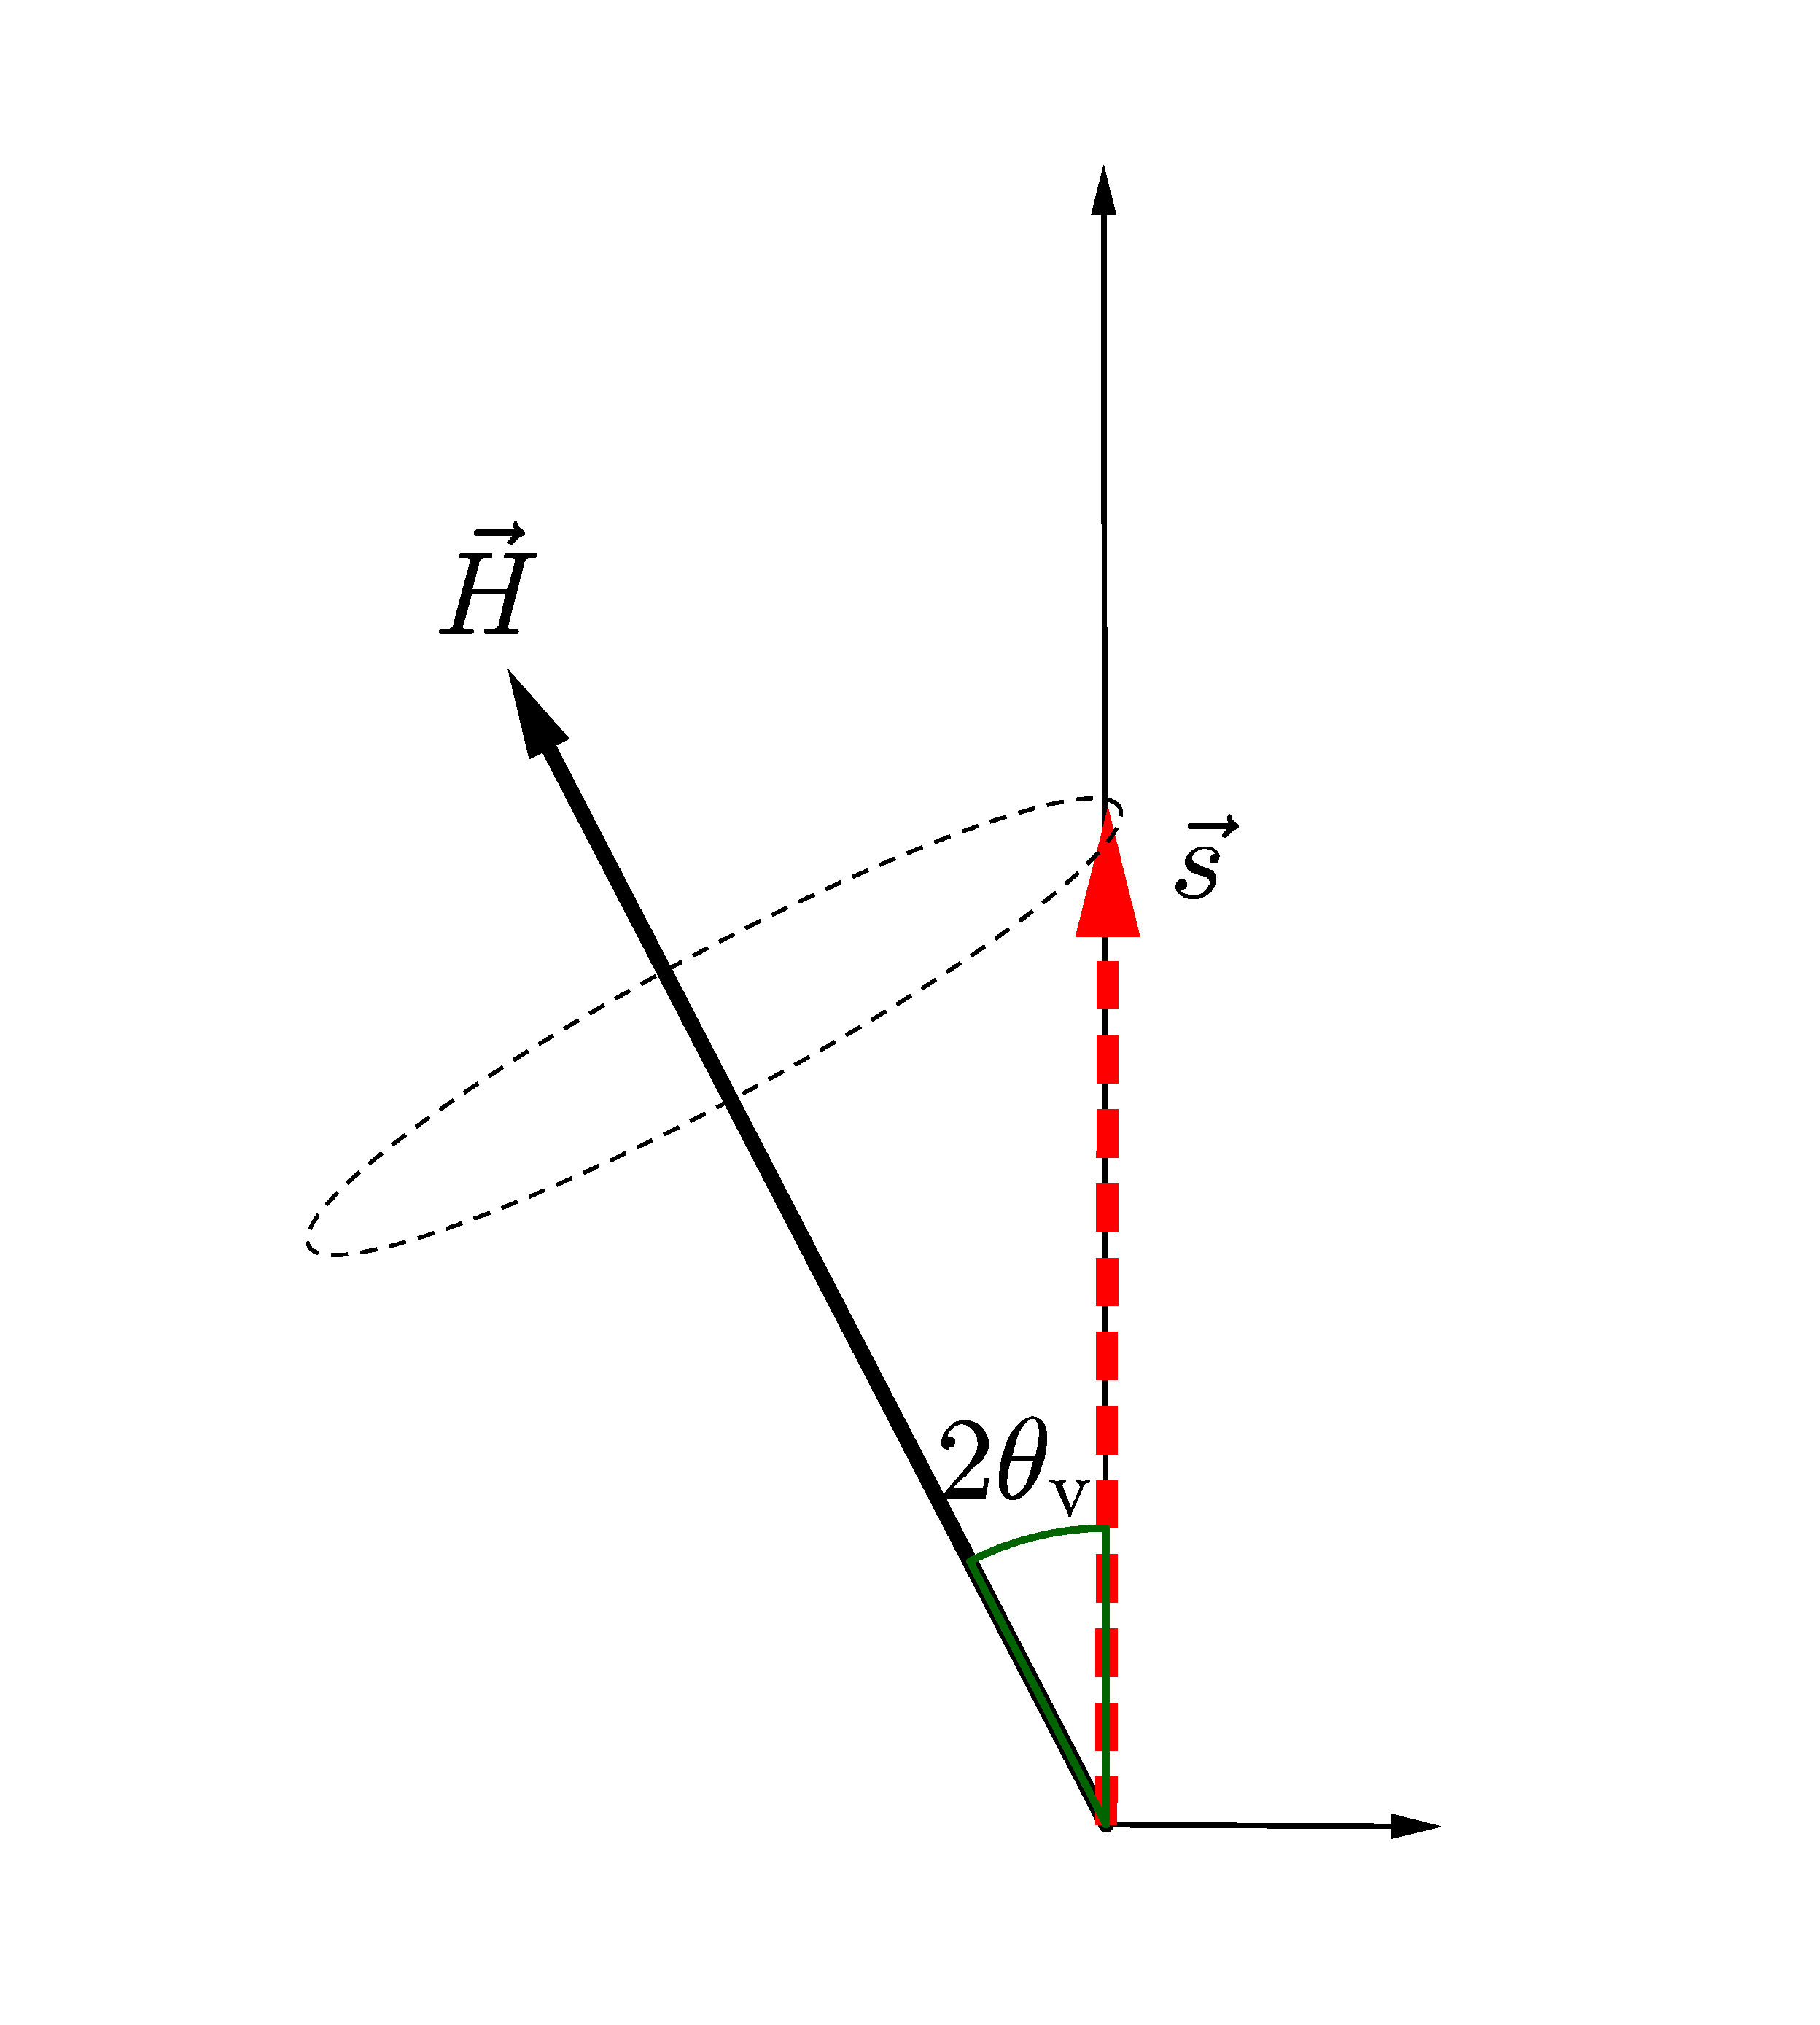
\includegraphics[width=0.7\textwidth]{assets/flavor-isospin-1}
\end{figure}
% \end{tcolorbox}



\end{column}
\end{columns}




\end{frame}
